\chapter{Methods}
\label{ch:methods}

\section{Introduction}

It is thought that the structure of the interstellar medium (ISM) plays a crucial role in the formation of stars and galaxies. The ISM is a complex and dynamic environment, characterized by a wide range of physical conditions, including temperature, density, and magnetic fields. Understanding the structure of the ISM is essential for understanding how stars and galaxies form and evolve.
Obsevations of the ISM reveal a rich tapestry of structures, ranging from small molecular clouds to large-scale filaments and bubbles. These structures are often characterized by their irregular shapes and complex geometries, which can make them difficult to analyze and interpret.
In this chapter, we will discuss the methods used to analyze the structure of the ISM, with a focus on the Minkowski functionals and the fractal dimension. These methods provide a powerful framework for quantifying the shape and structure of objects in a space, allowing us to derive various properties of the structures, such as their size, shape, and connectivity.

The fractal dimension is a measure of the complexity of the border of a shape, which can calculated using the Minkowski functionals.

\section{Minkowski Functionals}

The Minkowski functionals are a set of topological measures that can be used to quantify the shape and structures of objects in a space. From these functionals, we can derive various properties of the structures, such as their size, shape, and connectivity, but also connect .
These can be defined for any dimension, but we will focus on the 2D case, which is relevant for the analysis of the column density maps.

First it is convenient to define the concept of threshold, which is important both in understanding the methods but also in the application.
Excursion and Level Set: We define the excursion set $S_{\nu}$ of a given field on a $d$-dimensional domain $D \subset R^d$ as the set of points where $f$ exceeds a given threshold parameter $\nu$:

\begin{equation}
    S_{\nu} = \{ \mathbf{x} \in D : f(\mathbf{x}) > \nu \}
\end{equation}

The boundary of the excursion set is defined as the level set, which is the set of points where the field equals the threshold:

\begin{equation}
    \partial S_{\nu} = \{ \mathbf{x} \in D : f(\mathbf{x}) = \nu \}
\end{equation}

An example of these can be seen in Figure \ref{fig:level_set_example}.

\begin{figure}[t]
    \centering
    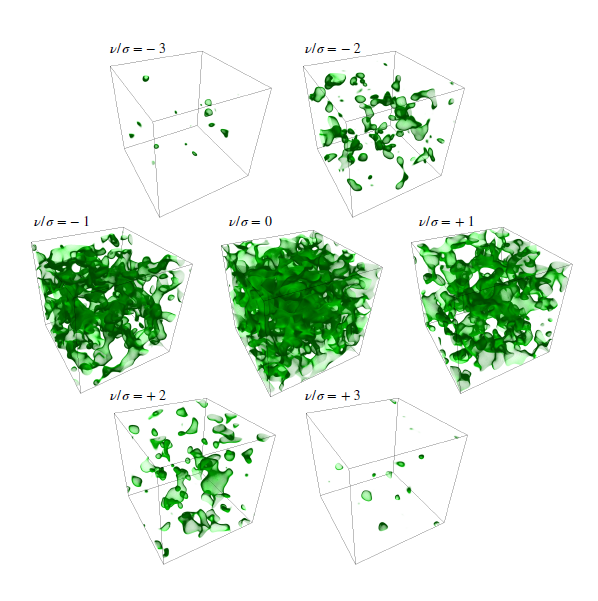
\includegraphics[width=0.6\textwidth]{figures/boundaries.png}
    \caption{Example of an excursion set and its boundary for a field for a smoothed three-dimensional Gaussian field.}
    \label{fig:level_set_example}
\end{figure}

The motion-invariants are defined as the integrals of the Minkowski functionals over the excursion set $S_{\nu}$, are d+1 and are called the Minkowski functionals. For a 2-dimensional map, these are:

\begin{itemize}
    \item $M_0(S_{\nu})$: the area of the excursion set, which is the integral of the field over the set $S_{\nu}$.
    \item $M_1(S_{\nu})$: the perimeter of the excursion set.
    \item $M_2(S_{\nu})$: the Euler characteristic of the excursion set, which is a measure of the connectivity of the set.
\end{itemize}

From these, we can define a lot of properties that can be calculated to characterize the structures in Orion A and B. 

The following section is divided into two parts: global properties and local properties. Global properties are those that describe the overall structure of the ISM, while local properties are those that describe how the structure changes as a function of column density.

\section{Global Properties}

\subsection{Global Fractal Dimension}

The fractal dimension is a measure of the border complexity of a given structure. This can be calculated using the Minkowski functionals, specifically the perimeter and area \cite{cannon1984fractal}. 
The main idea for this approach is that, for a given border length, a simple border will always enclose a larger area than a complex border.

On this idea, the perimeter-area (P-A) relation is defined as:

\begin{equation}
    \label{eq:perimeter_area}
    P = A^{\frac{D}{2}}
\end{equation}

By measuring the perimeter $P$ and area $A$ of a structure at different thresholds and fitting the logarithm of the perimeter to the logarithm of the area, we can derive the fractal dimension $D$ of the overall structure.

The relation between perimeter and area provides information about the complexity or degree of contortion of the boundary. For example, a fixed length of smooth, rounded perimeter can enclose a larger area than a highly irregular or convoluted perimeter. This degree of complexity can be characterized by the dimension $D$ of the perimeter. For smooth shapes, such as circles and squares, the scaling follows $P \propto A^{1/2}$, and thus $D=1$, corresponding to the dimension of a line. As the perimeter becomes increasingly contorted and tends to fold back on itself, effectively filling the plane, the scaling approaches $P \propto A$, and $D$ approaches a value of 2.

If the cloud exhibits structures with a well-defined length scale, we can consider the perimeter to be composed of large-scale features superimposed with small-scale noise or perturbations. In this case, the large- and small-scale structures would show different perimeter–area relations, and consequently, different values of $D$. Therefore, if the perimeter–area relation is characterized by multiple values of $D$ across scales, this would point to the existence of processes operating at characteristic spatial scales, and it would motivate a meaningful distinction between large- and small-scale structure. Conversely, if the perimeter–area relation is consistently described by a single power-law scaling, this indicates the absence of characteristic length scales in the cloud morphology.

Hence, if the linear fit in log–log space is robust, one can argue that the structure lacks a preferred scale and therefore behaves as a fractal. An example of this is illustrated in Figure~\ref{fig:perimeter_area_example}, where data from meteorological clouds were used to derive the fractal dimension of the structures. The slope of the linear fit yields the fractal dimension $D$, providing a quantitative measure of the structural complexity. The lack of a characteristic scale, evidenced by the good fit, suggests that turbulent processes are likely responsible for shaping the observed structures.

\begin{figure}[t]
    \centering
    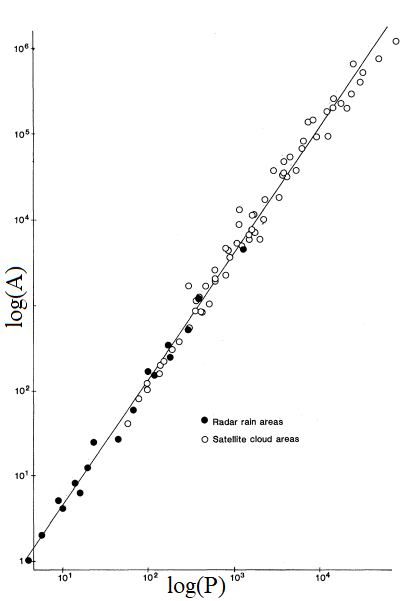
\includegraphics[width=0.4\textwidth]{figures/lovejoy.png}
    \caption{Example of the perimeter-area relation for meteorological clouds \cite{lovejoy1982area}. The slope of the linear fit gives the fractal dimension of the structure.}
    \label{fig:perimeter_area_example}
\end{figure}

This counts in this work a global property of the cloud.

The perimeter-area relation is a powerful tool for analyzing the complexity of structures in the ISM. It's simple, yet effective, and can be applied to a wide range of structures, from clouds to galaxies. The fractal dimension derived from the perimeter-area relation can provide insights into the physical processes that shape these structures, such as turbulence, gravity, and magnetic fields. It is also powerful to analyze the evolution of structures as a function of column density threshold.
However, it is important to note that the perimeter-area relation is not always applicable to all structures. Furthermore, numerical effects can also play a role in the calculation of the fractal dimension, as we will see in the simulations section. Artifacts also have an effect on this method \cite{imre2006artificial}. This is to say, that the method has its limitations and simulations play an important role in understanding these effects. 

\section{Local Properties}

\subsection{Local Fractal Dimension}

One further advantage of the perimeter–area relation is that it can be inverted to derive the fractal dimension of a structure at a given column density threshold. By inverting Eq.~\ref{eq:perimeter_area}, we can express the local fractal dimension $D$ as a function of the column density threshold $\nu$:

\begin{equation}
    \label{eq:local_fractal_dimension}
    D(\nu) = 2 \times \frac{\log\bigl(P(\nu)\bigr)}{\log\bigl(A(\nu)\bigr)}.
\end{equation}

This approach enables a more detailed characterization of the geometry and scaling behavior of the cloud structures as a function of physical conditions. In particular, by applying a series of increasing thresholds $\nu$, one effectively isolates progressively denser substructures within the molecular cloud. At each threshold, the perimeter $P(\nu)$ and area $A(\nu)$ can be measured either for all connected structures collectively or for each identified region individually.

In the first case, the perimeters and areas of all structures present in the map at a given threshold are summed, providing a global measurement of the local fractal dimension for that threshold. This yields a single $D(\nu)$ value for each column density level, capturing how the overall morphological complexity evolves as successively denser material is selected. An example of this approach is shown in Figure~\ref{fig:local_fractal_dimension_example}, where the perimeters and areas are computed across a range of thresholds, demonstrating the dependence of the fractal dimension on the chosen column density cut.

\begin{figure}[t]
    \centering
    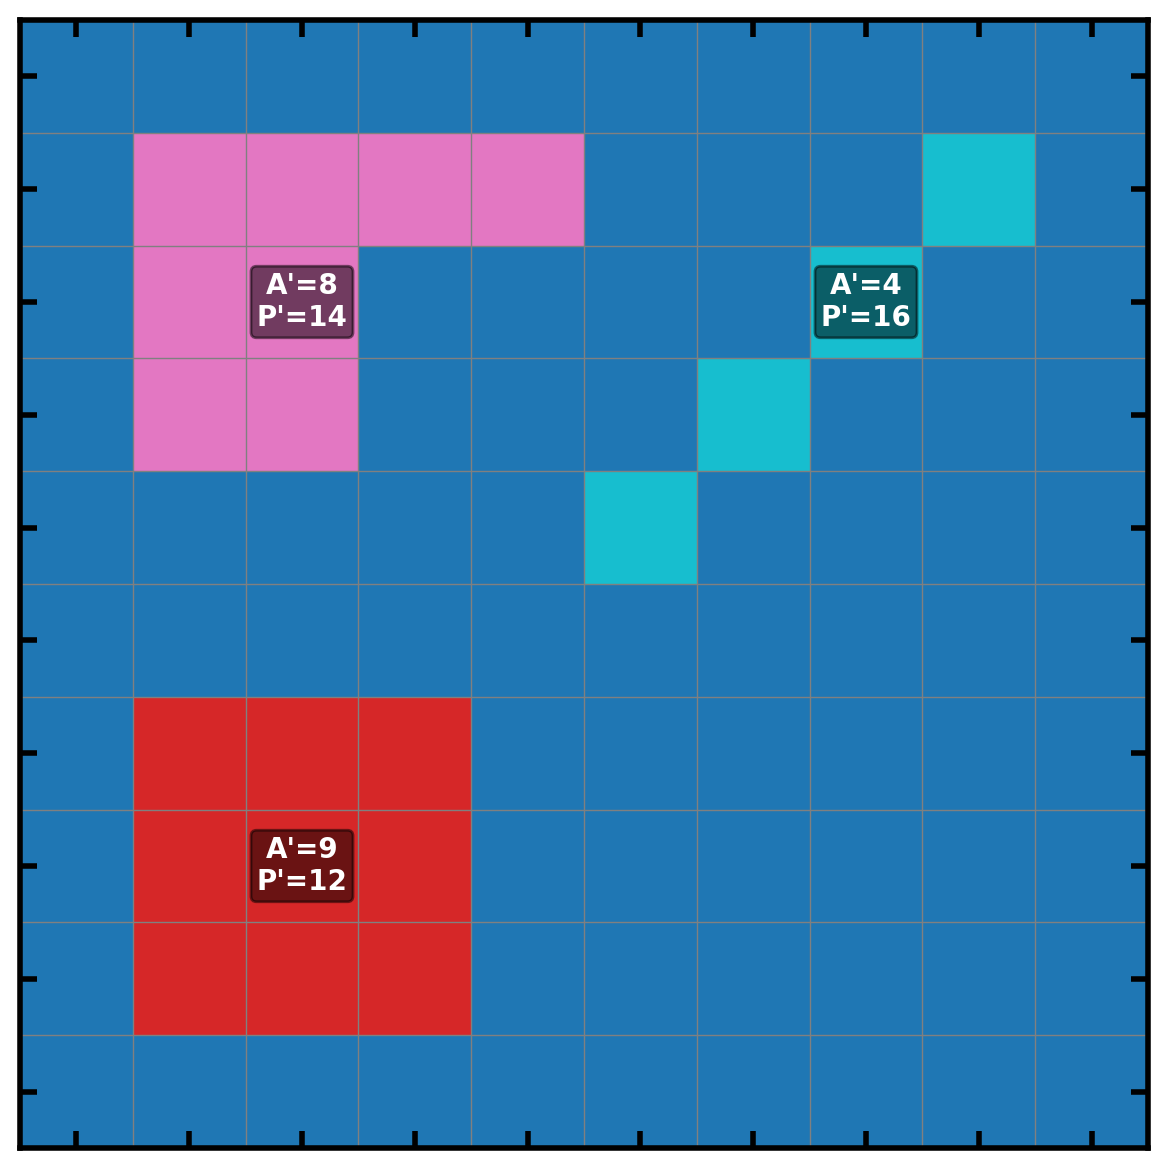
\includegraphics[width=0.5\textwidth]{figures/example_calculations.png}
    \caption{Simplified example of the calculation of perimeters and areas of structures at a given column density threshold. The local fractal dimension can be calculated by summing over all of the structures at that threshold, or for each of the single structures.}
    \label{fig:local_fractal_dimension_example}
\end{figure}

Conversely, it is also possible to calculate the local fractal dimension separately for each individual structure as a function of threshold. In this case, the evolution of $D$ with increasing density can be tracked on a per-object basis, providing insights into whether substructures become more or less fragmented and irregular as higher-density material is isolated. This allows the study of whether certain regions of the cloud exhibit self-similar scaling over a wide range of column densities, or whether there are transitions in the structural properties that may reflect different physical regimes, such as turbulence, gravitational collapse, or feedback from star formation.

Analyzing the local fractal dimension as a function of threshold thus provides a powerful tool to investigate the scale dependence and complexity of molecular clouds, complementing the global measurements and helping to disentangle the contributions from different physical processes.

\subsection{Dendrograms}

In order to explore the segmentation of structures with changing column density or mass, dendrograms are a useful tool. A dendrogram is a diagram that represents the hierarchical organization of structures within the data \cite{everitt2010cambridge}. Specifically, it shows how large-scale regions can be decomposed into smaller substructures as the threshold for the column density (or mass) increases.

By progressively applying higher thresholds, one can trace how individual dense clumps emerge from the diffuse background and how these clumps further fragment into even denser cores. In this way, dendrograms provide a visual and quantitative framework to analyze the nested, multiscale nature of molecular cloud structure.

In this work, dendrograms were constructed using hierarchical clustering methods applied to the mass maps of Orion A and B. This approach allows identification and characterization of the main branches (large coherent structures) as well as the terminal leaves (smallest resolved substructures). For each identified region, properties such as total mass, size (computed via principal component analysis), and fractal dimension were derived to quantify their physical characteristics and complexity.

\subsection{Mass-Size-Fractal Dimension (MSD) plane}

Since it is possible to calculate the local fractal dimension for single structure, we can connect this property to more physical aspects of the substructures, namely mass and size. This then allows us to include new information on mass-size diagrams, creating a Mass-Size-Fractal Dimension (MSD).

The dendrogram-like segmentation is an important aspect of this process, as it ensures a proper characterization and recognition of the sub-structures. 

\subsection{Euler characteristic}

Euler characteristic, often denoted as $\chi$ or $M_2(S_{\nu})$, and in two dimensions it is given by:
\begin{equation}
    \chi = \text{Number of connected regions} - \text{Number of holes}
\end{equation}
For a given excursion set $S_{\nu}$, the Euler characteristic provides a measure of the topology of the structures, indicating how many isolated regions and holes are present at a specific threshold. In practice, a positive Euler characteristic indicates more isolated regions than holes, while a negative value suggests a topology dominated by holes.

The Euler characteristic is closely related to the genus $G$ of the structure, where in two dimensions $G = 1 - \chi$. The genus is commonly used in cosmology and astrophysics to describe the connectivity of structures, such as the filamentary network in the ISM or the cosmic web. By analyzing the Euler characteristic or genus as a function of the threshold, one can gain insights into the morphological transitions and connectivity of the observed structures.

\section{Connection to star formation}

TBD

\section{Simulations}

% more details
\subsection{Simulations for the Global Properties}

The simulations addressing the global properties are primarily designed to verify the interpretation of the values obtained for the global fractal dimension $D$, as described in the preceding sections. In particular, they aim to confirm the expectation that the perimeter–area relation should yield unreliable or systematically biased results for structures that possess a well-defined characteristic length scale. 

In this context, Gaussian Random Fields (GRFs) play an important role as a benchmark for comparison. GRFs allow the generation of synthetic structures with controlled statistical properties and scaling behavior, providing a framework to test whether the methodology is sensitive to the presence or absence of intrinsic scales.

\subsection{Simulations for the Local Properties}

Analogously, simulations are employed to better understand how different values of the local fractal dimension arise in different types of structures. These tests include the analysis of Gaussian Random Fields, purely Gaussian noise, and simple geometric shapes such as lines and circles. 

The simulations also allow for quantifying numerical effects and resolution-dependent biases, assessing how limited spatial resolution and discretization influence the measured properties of the identified structures. This helps ensure that the interpretation of the fractal dimension is robust and not merely an artifact of the analysis method or data sampling.

\subsection{Comparison with Other Methods}

In the context of the simulations, a brief comparison with alternative approaches was carried out. This served both to improve understanding of the fractal dimension framework and to identify potential limitations or artifacts of the perimeter–area (PA) method.

The method most frequently used for comparison was the box-counting technique, which relies on covering the shape with a grid of boxes of varying sizes and counting the number of boxes that contain part of the shape. By examining how this count scales with the box size, the fractal dimension can be estimated \cite{falconer2013fractal}. 

\section{Uncertainties}

% Probs need to describe how to go from sigma_P and sigma_A to sigma_D ...
\subsection{Perimeter and Area}

The measurement of perimeter and area is subject to inherent uncertainties. To estimate these uncertainties, the following procedure was carried out:

\begin{itemize}
    \item The perimeter ($P$) and area ($A$) were measured for a set of circles with known true perimeter and area.
    \item The magnitude of the measurement error was computed by comparing the measured values to the true values.
    \item The errors were averaged over a sufficiently large number of samples ($N$) to obtain representative estimates of the typical deviation.
\end{itemize}

\subsection{Beam Size}

The finite resolution imposed by the telescope beam introduces systematic uncertainties in the measurement of structural properties. The beam convolution smooths small-scale fluctuations and reduces the complexity of the contour at each column density threshold. This effect generally leads to an underestimation of the perimeter and an overestimation of the area, biasing the derived fractal dimension toward lower values.

To quantify this uncertainty, one can simulate synthetic column density maps with known fractal characteristics and convolve them with a Gaussian kernel matching the observational beam. By comparing the perimeter–area relations before and after convolution, the bias introduced by the finite resolution can be estimated. Alternatively, the characteristic beam size provides a natural lower limit to the spatial scales where fractal analysis is reliable. In this work, scales smaller than 2–3 times the beam full-width at half-maximum (FWHM) are treated with caution, and the derived fractal dimensions are interpreted as lower limits to the intrinsic complexity of the cloud morphology.

\subsection{Uncertainties in the Extinction Map}

The dataset also includes a pixel-wise $\tau_{850}$ error map, as shown in Figure \ref{fig:error_map}. 

\begin{figure}[t]
    \centering
    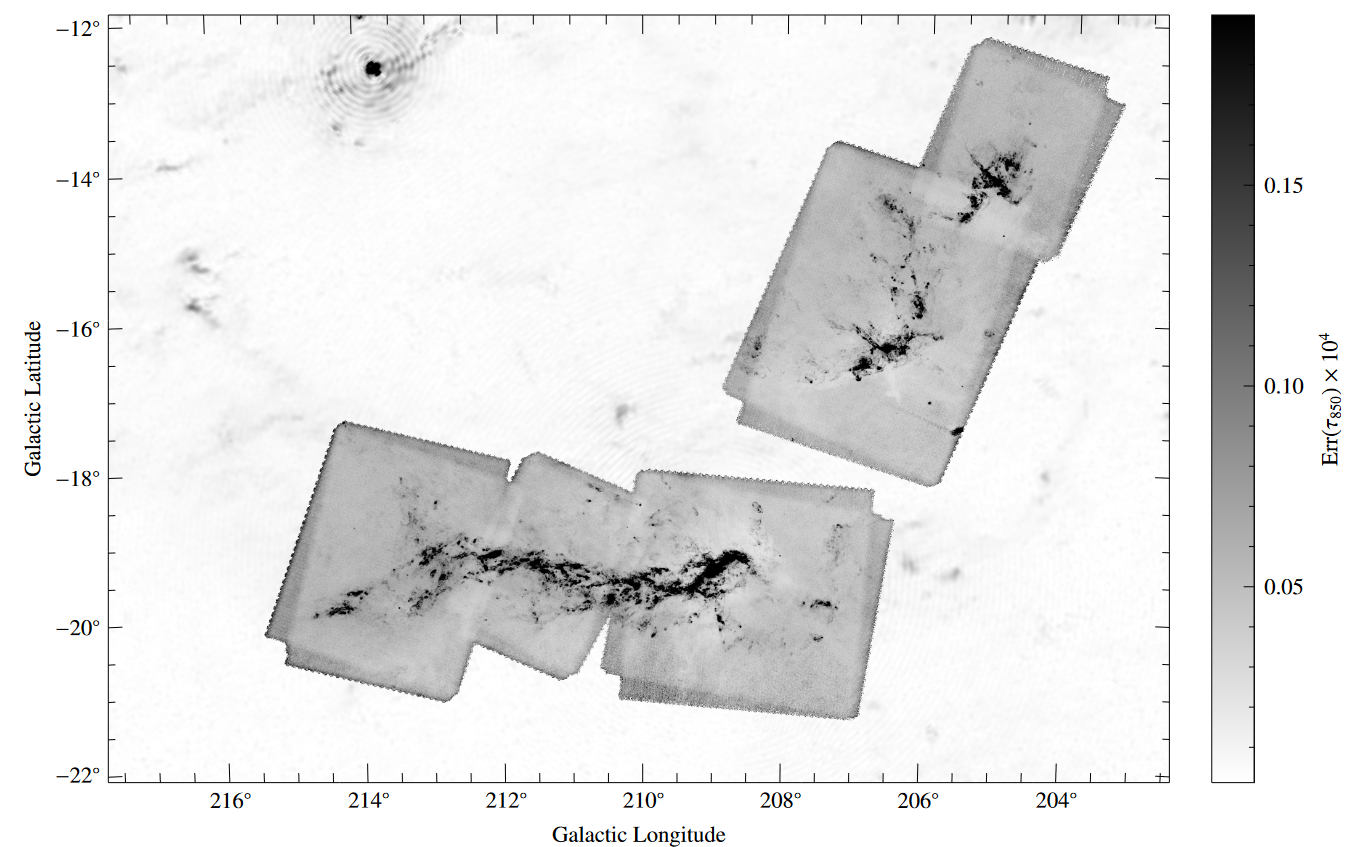
\includegraphics[width=0.75\textwidth]{figures/error_map.png}
    \caption{Pixel-wise error map of the $\tau_{850}$ data \cite{lombardi2014herschel}}
    \label{fig:error_map}
\end{figure}

Although these uncertainties are of a non-negligble magnitude to other sources of error and, in principle, all effects should be taken into account, the dominant contributions to the total uncertainty arise from the measurements of perimeter and area. 
For this reason, the pixel-wise extinction errors are neglected in the following analysis.
